\documentclass[11pt,a4paper,english]{article}
\usepackage[english]{babel}
\usepackage[utf8]{inputenc}
\usepackage{amsmath,amsfonts,amssymb,graphicx,textcomp,caption,color,listings,subcaption}
\usepackage[T1]{fontenc}
\usepackage[section]{placeins}
\usepackage[hidelinks,bookmarksnumbered]{hyperref}
\usepackage[all]{hypcap}
\usepackage[top=1in]{geometry}
\renewcommand{\thesubsection}{\thesection.\alph{subsection}}

\title{Nettbutikk documentation}
\author{Kristian Nilsen, Jon Erik Ullvang, Vinh Laph Nguyen,\\ Katharina Unstad, Espen Sotnakk}

\begin{document}
\maketitle
\fontfamily{ptm}\selectfont
\section*{Home}
This is the shop homepage where the products are shown as shown in Figure~\ref{fig:home}. Pressing on an item will open a modal showing more information and an button to add the item to cart.
\begin{figure}[htbp]
  \centering
  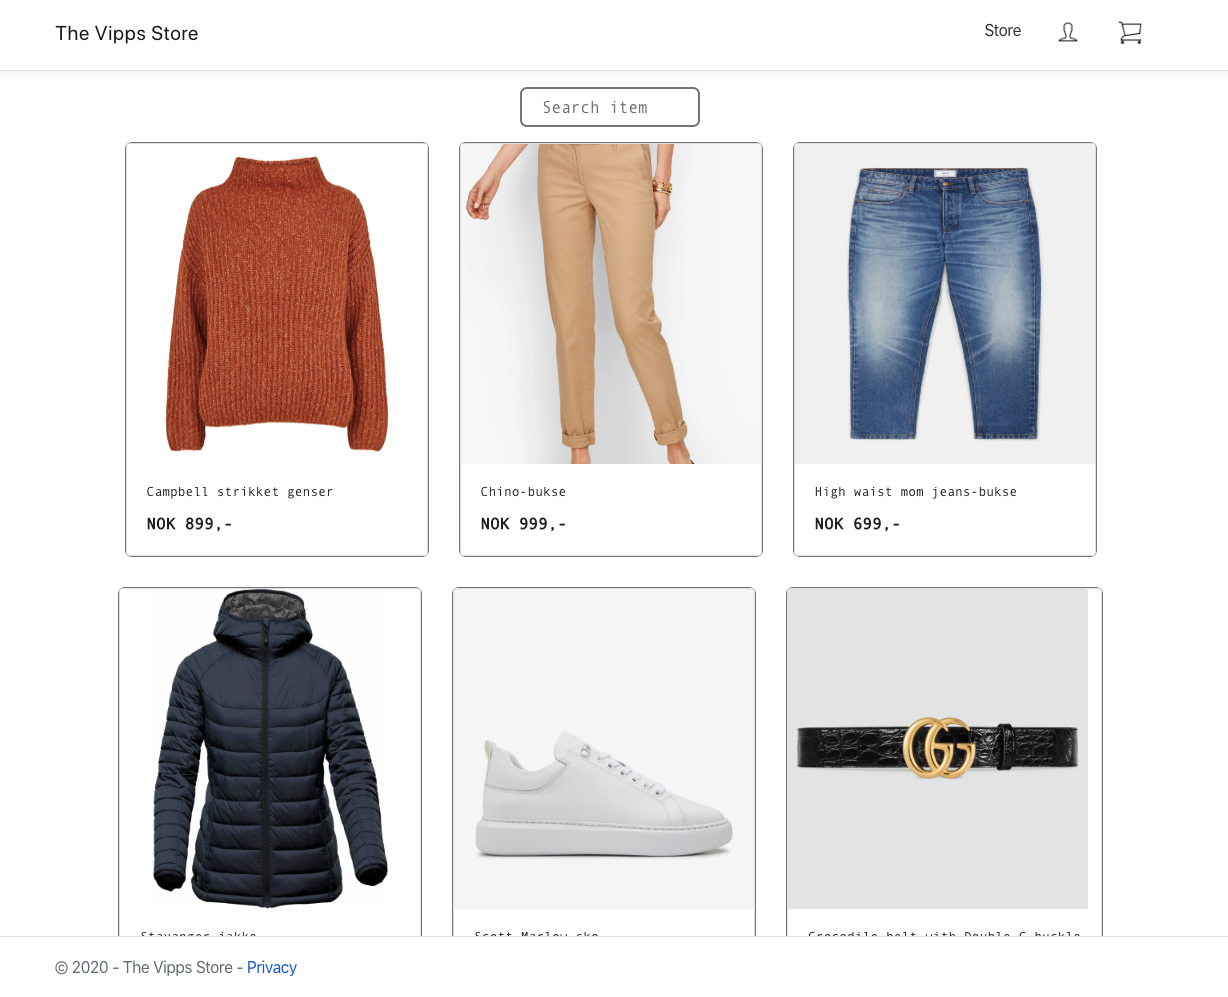
\includegraphics[scale=0.2]{home}
  \caption{Shop homepage showing products in a grid.}
  \label{fig:home}
\end{figure}
\section*{Product}
This modal opens when the product is pressed as shown in Figure~\ref{fig:item}. The modal shows more information about the item and a button to add item to cart. Pressing the x in the top left corner or pressing outside of the modal closes modal, and the home page is shown again.
\begin{figure}[htbp]
  \centering
  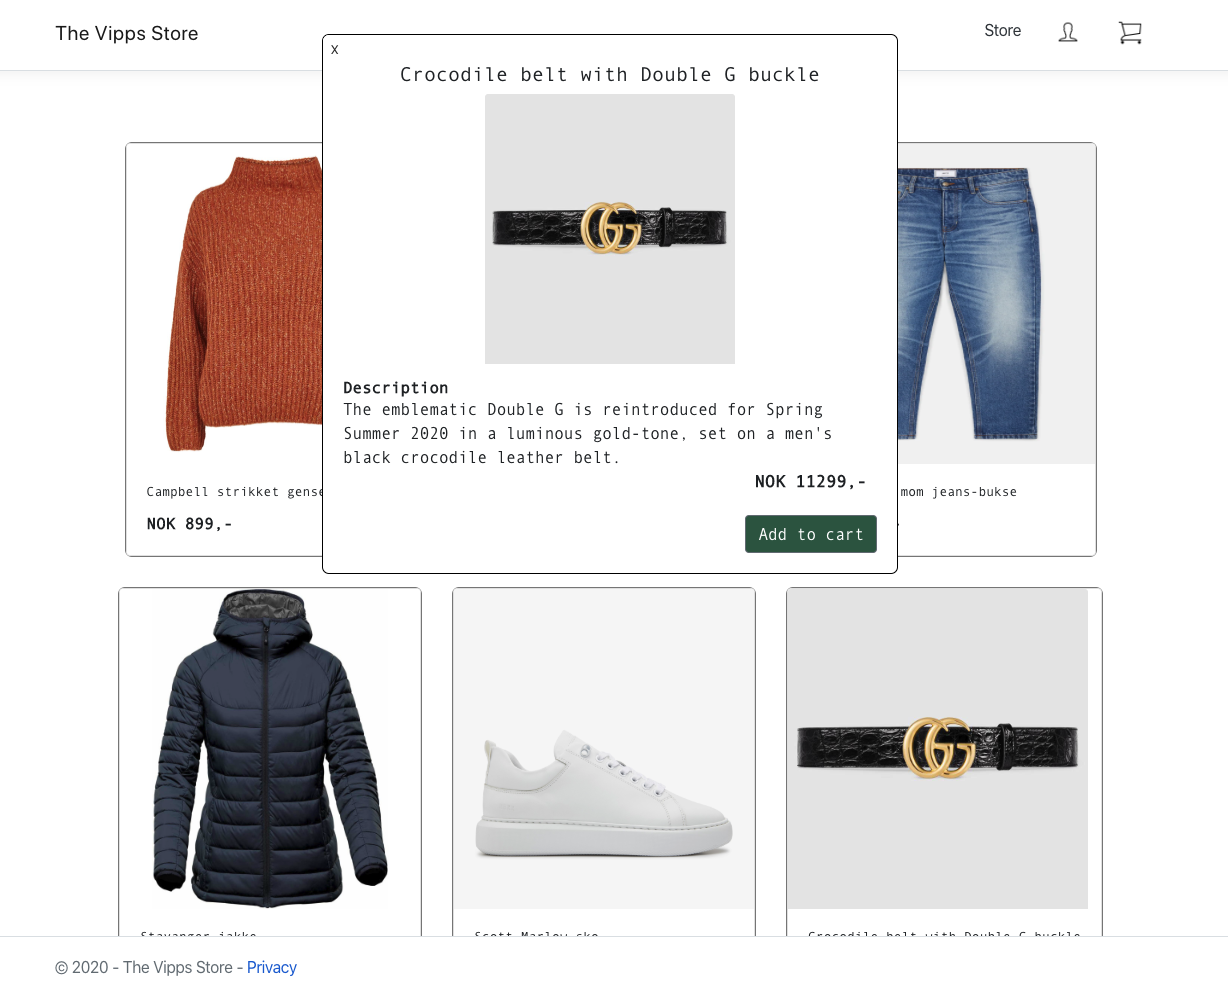
\includegraphics[scale=0.2]{item}
  \caption{Modal showing the product information.}
  \label{fig:item}
\end{figure}
\section*{Cart}
The cart page is shown in Figure~\ref{fig:cart} and shows a list of the items added to cart. Each item has a button to remove the item from cart. A sum of the amount for the items added to cart is shown with a button to continue to order page.
\begin{figure}[htbp]
  \centering
  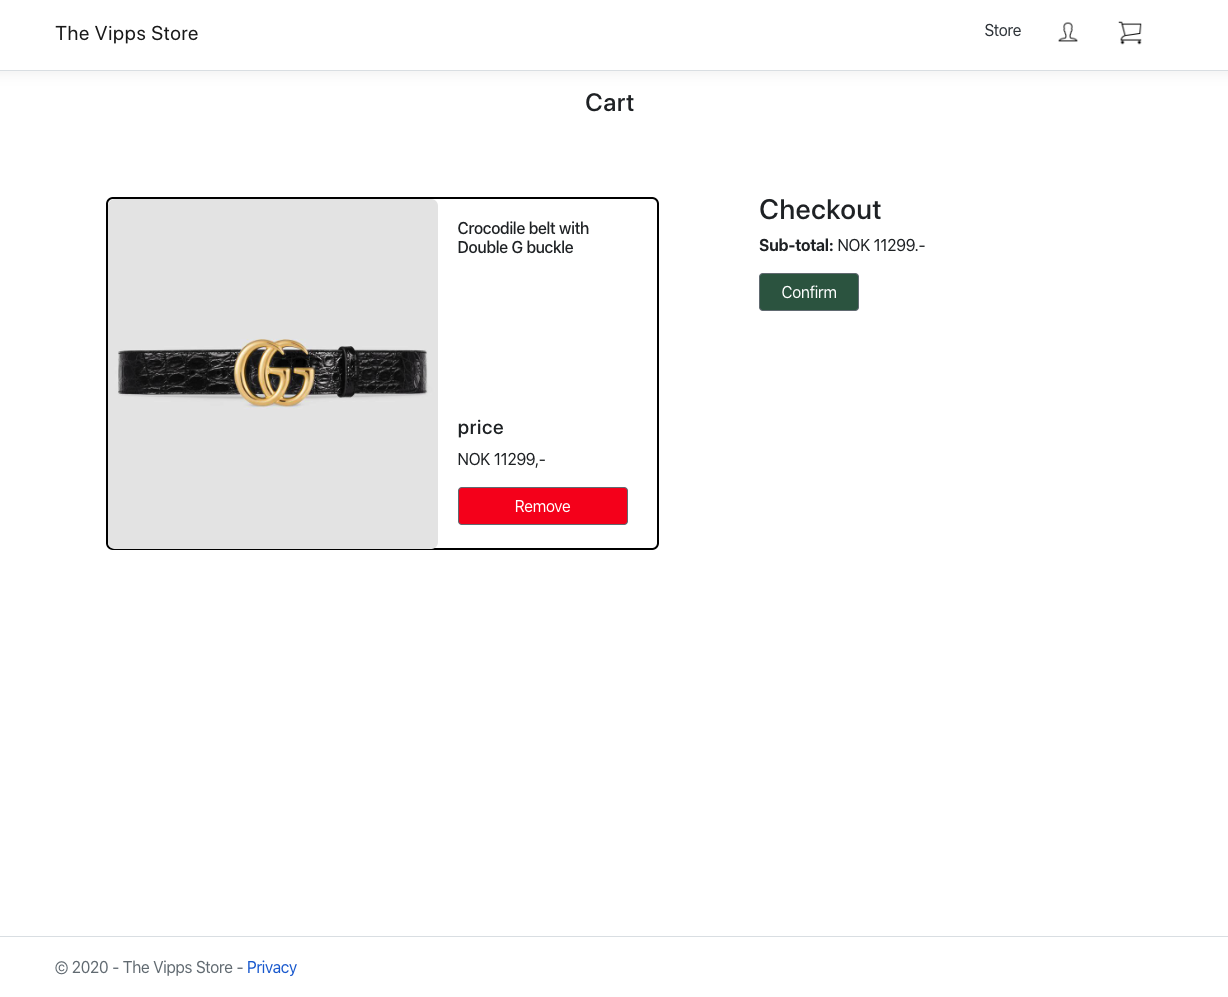
\includegraphics[scale=0.2]{cart}
  \caption{}
  \label{fig:cart}
\end{figure}
\section*{Order details}
This is the page where the users fills in information for placing an order. All fields are required with valid data.
\begin{figure}[htbp]
  \centering
  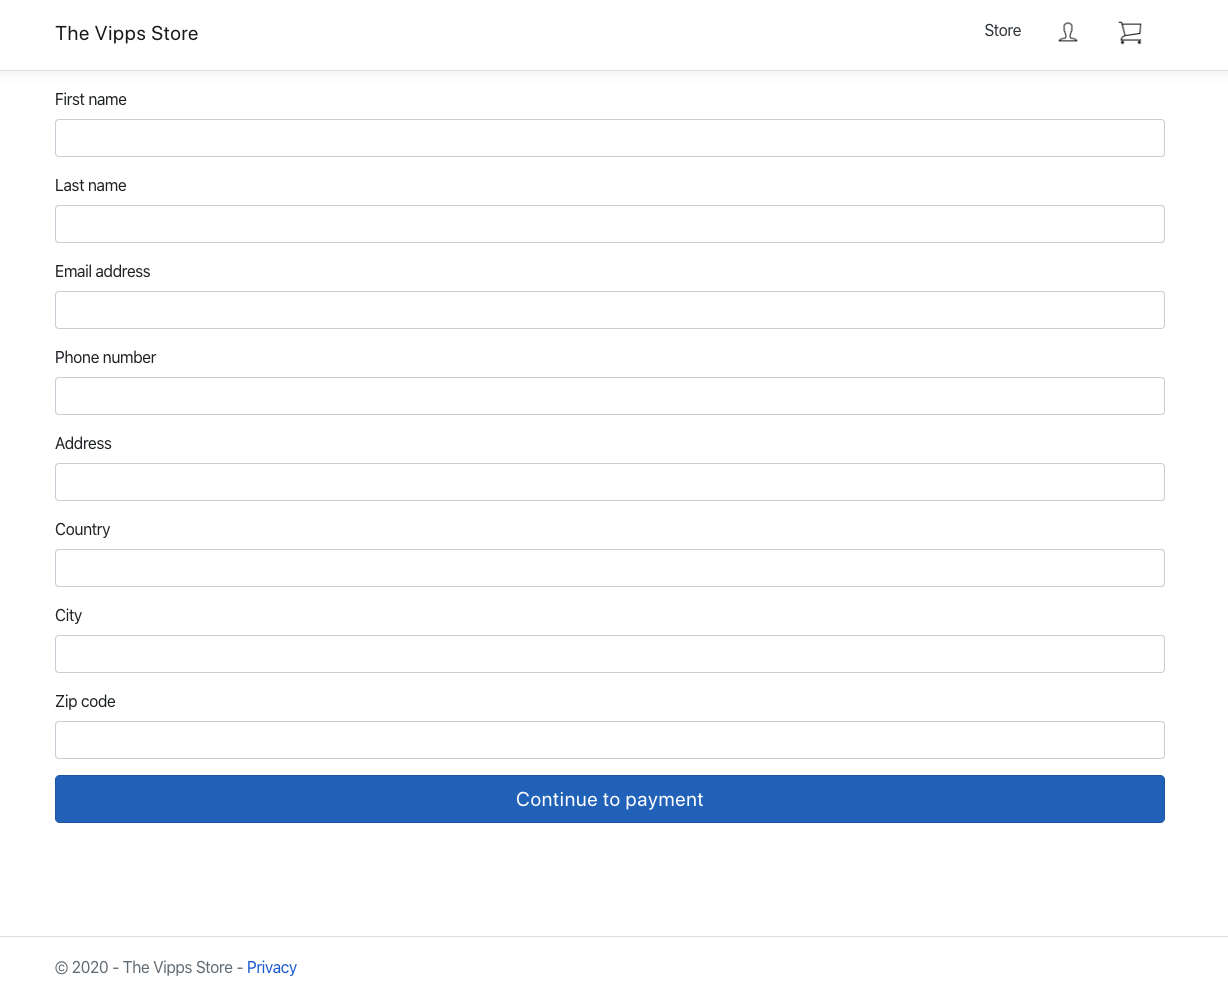
\includegraphics[scale=0.2]{order}
  \caption{Shows the form required for making an order.}
  \label{fig:order}
\end{figure}
\section*{Register}
Register page is shown in Figure~\ref{fig:register}. There are two options for registering a new account. One is to create user with email and password. The other option is to use facebook. Account confirmation is required after registering a new user. The user will be routed to a screen where they can enable two factor authentication which is recommended.
\begin{figure}[htbp]
  \centering
  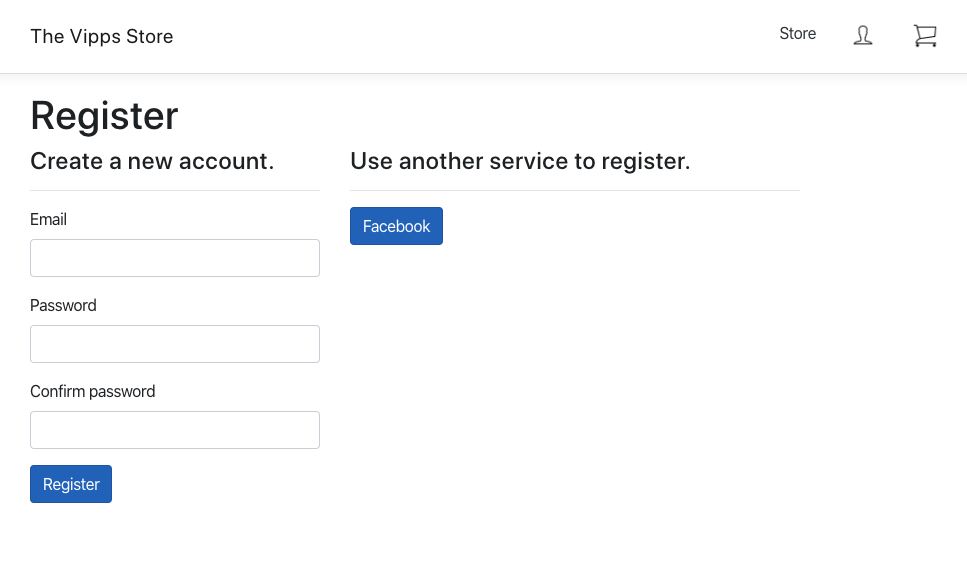
\includegraphics[scale=0.3]{register}
  \caption{Register page.}
  \label{fig:register}
\end{figure}
\section*{Login}
The login page is shown in Figure~\ref{fig:login}. The user has two options to login. The first is with an account the user created. The other is with authenticate with facebook.
\begin{figure}[htbp]
  \centering
  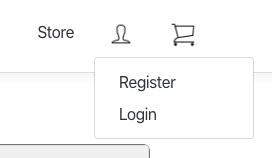
\includegraphics[scale=0.3]{login}
  \caption{Login page.}
  \label{fig:login}
\end{figure}
\section*{Payment}
The payment modal is shown in Figure~\ref{fig:stripe}. Here the customer inputs card information.
\begin{figure}[htbp]
  \centering
  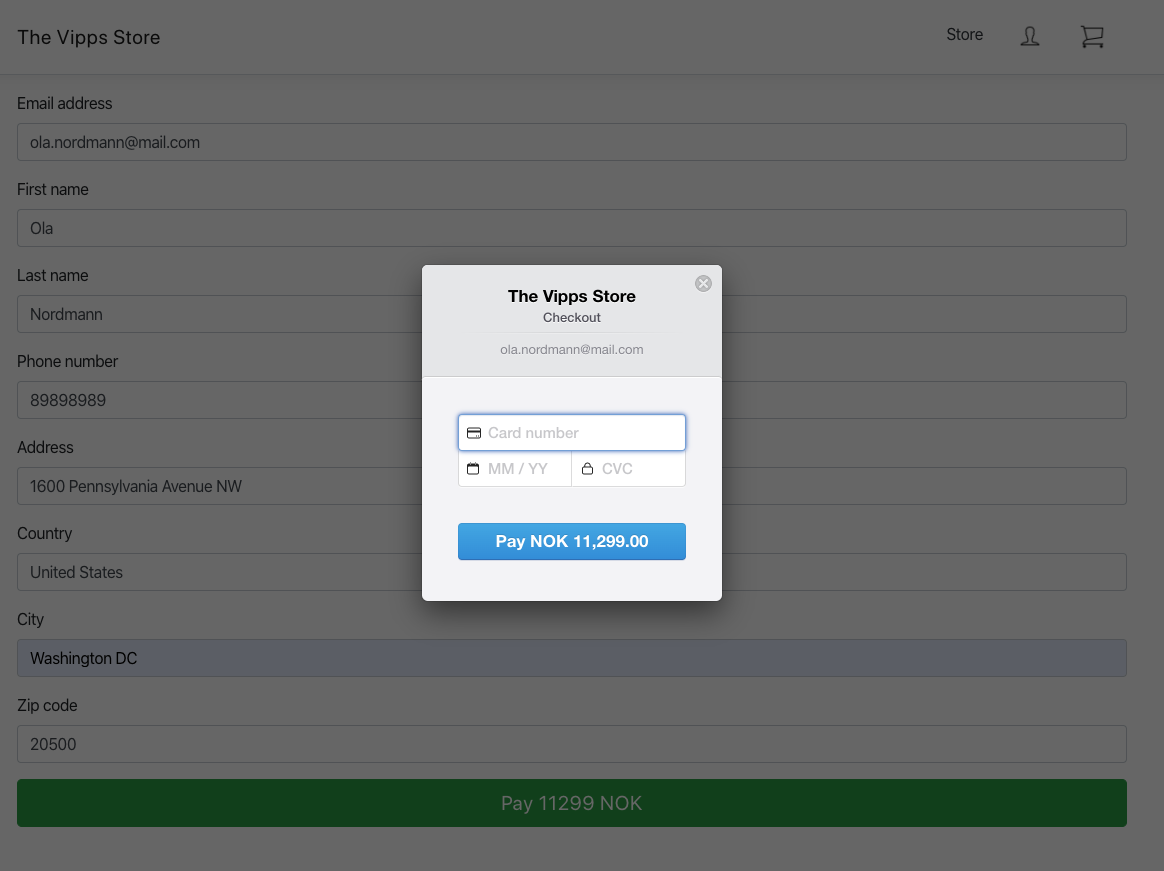
\includegraphics[scale=0.3]{stripe}
  \caption{Payment processing.}
  \label{fig:stripe}
\end{figure}
\section*{Order history}
Order history is shown in Figure~\ref{fig:history}. This is where orders placed by the user is shown. Clicking on an order shows additional information for that order as shown in Figure~\ref{fig:historydetails}.
\begin{figure}[htbp]
  \centering
  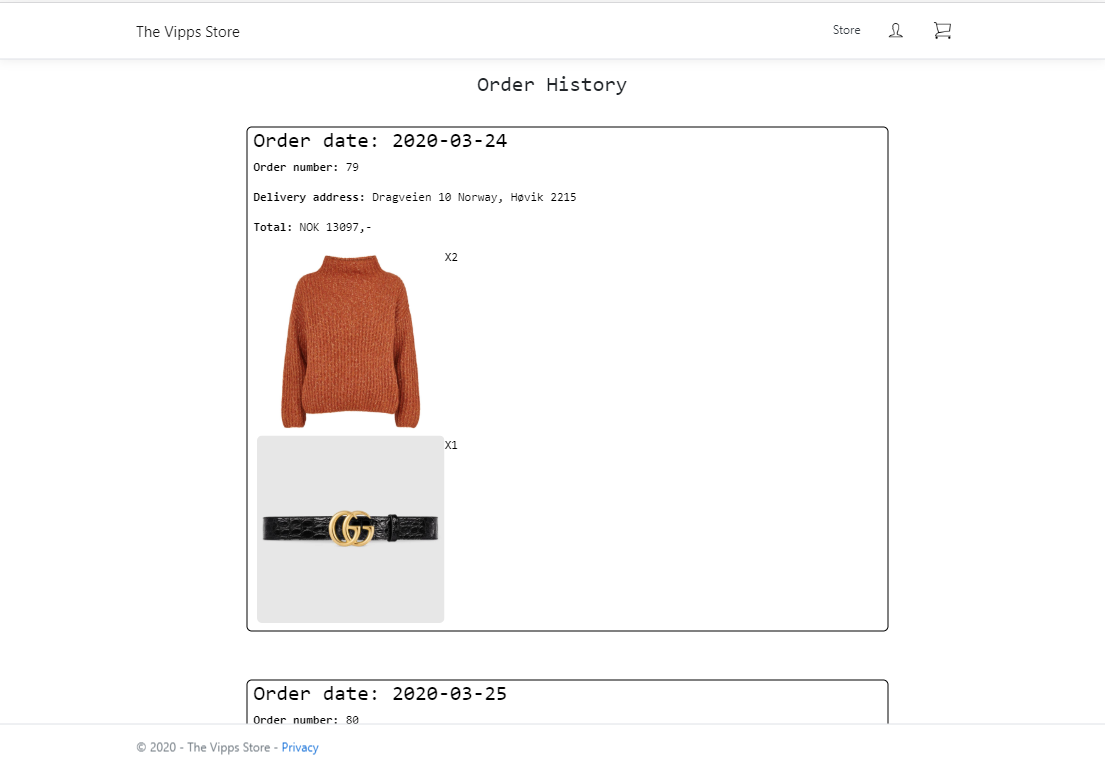
\includegraphics[scale=0.3]{orderhistory}
  \caption{Order history page.}
  \label{fig:history}
\end{figure}
\begin{figure}[htbp]
  \centering
  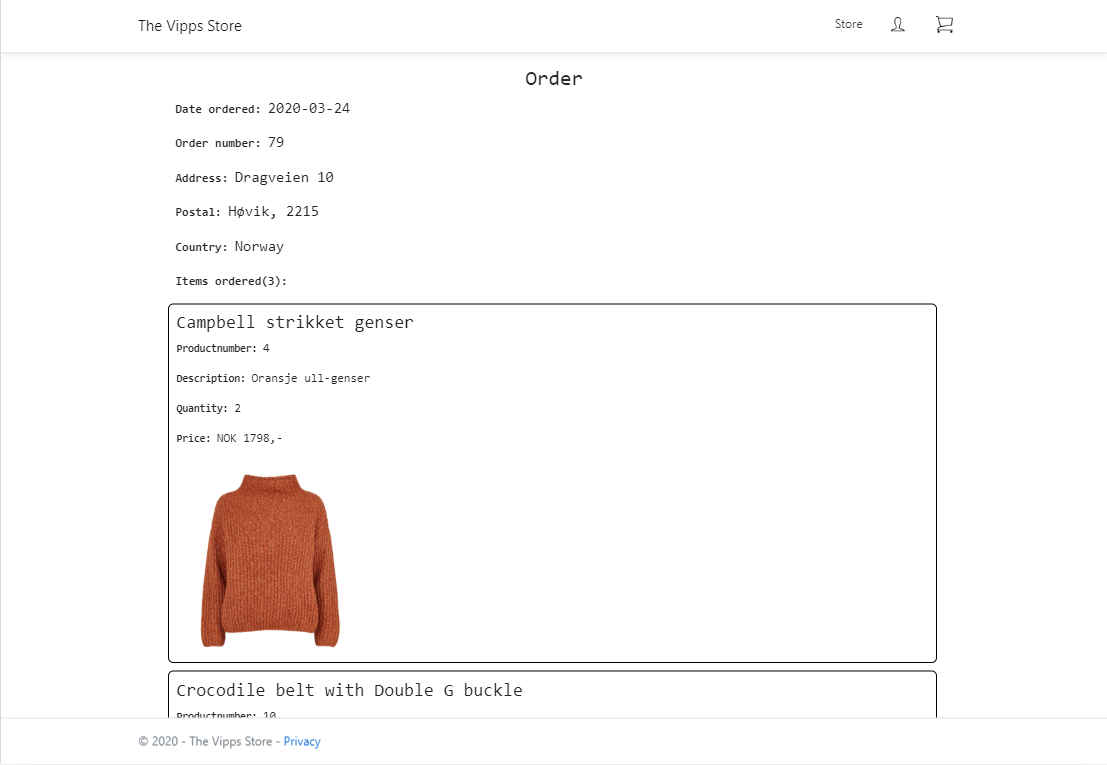
\includegraphics[scale=0.3]{orderhistorydetails}
  \caption{Order details.}
  \label{fig:historydetails}
\end{figure}
\section*{Profile page}
The profile page is shown in Figure~\ref{fig:profile}. On this page the user can write in profile details. This information will be used in the order details page when the customers proceeds from the cart. The user is able to change any information for the order on the page.
\begin{figure}[htbp]
  \centering
  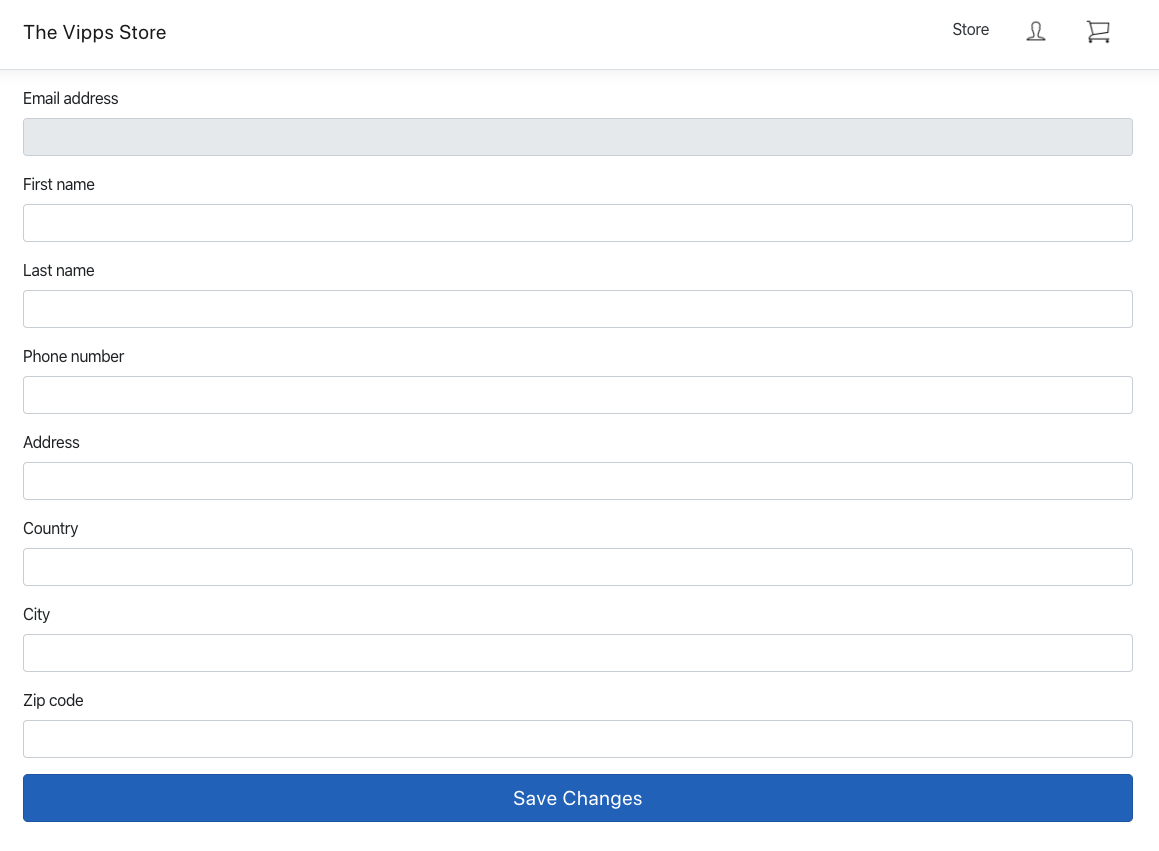
\includegraphics[scale=0.2]{profile}
  \caption{Order details.}
  \label{fig:profile}
\end{figure}
\end{document}
